\documentclass[11pt]{article}

\usepackage{fullpage}
\usepackage{graphicx}
\usepackage{amsmath}
\usepackage{amssymb}
\usepackage{amsthm}
\usepackage{fancyvrb}

\parindent0in
\pagestyle{plain}
\thispagestyle{plain}

\newcommand{\myname}{Mehshan Mustafa}
\newcommand{\dated}{\today}

\newenvironment{theorem}[2][Theorem]{\begin{trivlist}
\item[\hskip \labelsep {\bfseries #1}\hskip \labelsep {\bfseries #2.}]}{\end{trivlist}}
\newenvironment{lemma}[2][Lemma]{\begin{trivlist}
\item[\hskip \labelsep {\bfseries #1}\hskip \labelsep {\bfseries #2.}]}{\end{trivlist}}
\newenvironment{exercise}[2][Exercise]{\begin{trivlist}
\item[\hskip \labelsep {\bfseries #1}\hskip \labelsep {\bfseries #2.}]}{\end{trivlist}}
\newenvironment{problem}[2][Problem]{\begin{trivlist}
\item[\hskip \labelsep {\bfseries #1}\hskip \labelsep {\bfseries #2.}]}{\end{trivlist}}
\newenvironment{question}[2][Question]{\begin{trivlist}
\item[\hskip \labelsep {\bfseries #1}\hskip \labelsep {\bfseries #2.}]}{\end{trivlist}}
\newenvironment{corollary}[2][Corollary]{\begin{trivlist}
\item[\hskip \labelsep {\bfseries #1}\hskip \labelsep {\bfseries #2.}]}{\end{trivlist}}
\newenvironment{solution}{\begin{proof}[Solution]}{\end{proof}}
\newenvironment{idea}[2][Proof Idea.]{\textit{#1} #2}

\begin{document}
\textbf{Introduction to the Theory of
Computation}\hfill\textbf{\myname}\\[0.01in]
\textbf{Chapter 1: Reqular Languages}\hfill\textbf{\dated}\\
\smallskip\hrule\bigskip

\begin{problem}{1.31}
Let $B_{n} = \{a^{k} \ | \ k \ is \ a \ multiple \ of \ n \}$. Show that for each $n \geq 1$, the language $B_{n}$ is regular.
\end{problem}

\begin{idea}
$B_{1} = \{\epsilon, a, aa, aaa, aaaa, \cdots \}$ and $B_{3} = \{\epsilon, aaa, aaaaaa, aaaaaaaaa, \cdots \}$.
\begin{center}
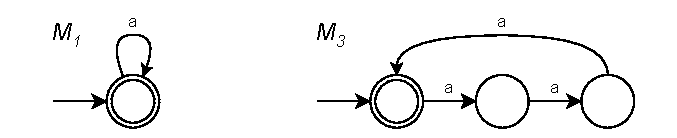
\includegraphics[scale=1.0]{Figures/Problem1.36.pdf} \\
State diagrams of DFAs that recognize $B_{1}$ and $B_{3}$.
\end{center}
\end{idea}

\begin{proof}
The proof is by construction. Construct the DFA $M_{n} = (Q, \Sigma, \delta, q_{0}, F)$ to recognize $B_{n}$:
\begin{enumerate}
\item $Q = \{q_{1}, q_{2}, q_{3}, \cdots, q_{n}\}$, where $n \geq 1$.
\item $\Sigma = \{a\}$
\item $q_{0} = q_{1}$
\item $F = \lbrace q_{1} \rbrace$
\item Define $\delta$(q, a) so that for any $q \in Q$ and any $a \in \Sigma$:
\end{enumerate}
\begin{center}
$\displaystyle \delta( q,\ a) \ =\begin{cases}
q_{i+1} & 1 \leq i < n \\
q_{1} & i = n \\
\end{cases} \ \ $
\end{center}
\end{proof}
\end{document}